\documentclass[aspectratio=169]{beamer} % Aspect ratio 16:9 para pantallas modernas
\usepackage[utf8]{inputenc}
\usepackage[T1]{fontenc}
\usepackage[spanish, es-tabla]{babel}
\usepackage{helvet}
\usepackage{amsmath, amssymb, amsthm}
\usepackage{graphicx} 
\usepackage{booktabs}
\usepackage{tikz} 
\usepackage{graphicx}
\usepackage{hyperref}
\usetikzlibrary{arrows.meta, positioning, automata}
\usetheme{UNAM}

\title{Optimización II}
\subtitle{Práctica: Rutas más Cortas y Flujo Máximo}
\author{Ricardo López Ramírez \and Emiliano Sanchez Ruiz}
\date{\today}
\institute{\url{423092556@pcpuma.acatlan.unam.com.mx}}

\begin{document}

\begin{frame}[plain,t]
    \titlepage
\end{frame}

\begin{frame}
    \frametitle{Índice}
    \tableofcontents
\end{frame}


\section{Introducción y Objetivo}

\begin{frame}
    \frametitle{Introducción y Planteamiento}
    \textbf{Situación de Análisis: Red del Bosque}
  
    Se modeló la red peatonal del parque definiendo los siguientes parámetros:
    \begin{itemize}
        \item \textbf{Nodos (15):} Puntos de interés (N1: Lago, N15: Aviario, etc.)
        \item \textbf{Arcos (32):} Senderos que conectan las atracciones.
        \item \textbf{Costos ($c_{ij}$):} Distancia física en metros de cada sendero.
    \end{itemize}
    \vspace{0.2cm}
    \textbf{Objetivos del Análisis (Dos aplicaciones):}
    \begin{enumerate}
        \item \textbf{Ruta Más Corta (Dijkstra):} Hallar el trayecto mínimo de N1 a N15 para vehículos de emergencia, incluyendo su formulación en Programación Lineal.
        \item \textbf{Rutas entre Todo Par de Nodos (Floyd-Warshall):} Generar una matriz global de distancias para crear mapas y señalética para los visitantes.
    \end{enumerate}
\end{frame}

\section{Ubicación Nodos y APP}
\begin{frame}{Ubicación de los Nodos}
    \begin{table}[]
        \centering
        \small
        \begin{tabular}{cl|cl|cl}
            \toprule
            \textbf{ID} & \textbf{Lugar} & \textbf{ID} & \textbf{Lugar} & \textbf{ID} & \textbf{Lugar} \\
            \midrule
            \textbf{N1} & Lago & \textbf{N6} & Herpetario & \textbf{N11} & Ahuehuete \\
            \textbf{N2} & Casa del Lago & \textbf{N7} & Jardín Botánico & \textbf{N12} & Semi Lago \\
            \textbf{N3} & Zoo Aventuras & \textbf{N8} & Orquideario & \textbf{N13} & F. Quijote \\
            \textbf{N4} & Zoológico & \textbf{N9} & Castillo & \textbf{N14} & Sor Juana \\
            \textbf{N5} & Museo Axolote & \textbf{N10} & (Nodo Central) & \textbf{N15} & Aviario \\
            \bottomrule
        \end{tabular}
    \end{table}

    \frametitle{Aplicación Web}

    \begin{center}
        \href{https://enfrentamientoboochapultepec-jlwmnf4kxphwckqebymu5w.streamlit.app/}
        {\beamerbutton{Abrir Aplicación}}
    \end{center}
    
\end{frame}


\section{Objetivos del Análisis}
\begin{frame}{Objetivos del Análisis}
    \textbf{Objetivo General:}
    Optimizar la movilidad y logística de los visitantes dentro del parque.
    \vspace{0.5cm}
    
    \textbf{Objetivos Específicos:}
    \begin{enumerate}
        \item \textbf{Ruta Más Corta (Dijkstra/Floyd):} Determinar el camino de menor distancia (en metros) para que un vehículo de emergencia o carrito de rescate se desplace desde el \textbf{N1 (Lago)} hasta el \textbf{N15 (Aviario)}.
        \vspace{0.2cm}
        \item \textbf{Flujo Máximo (Ford-Fulkerson):} En caso de una evacuación coordinada, determinar la cantidad máxima de personas por minuto que la red de senderos puede transportar desde el \textbf{N1} hasta las puertas de salida en el \textbf{N15}, evitando embotellamientos y respetando la capacidad de las vías.
    \end{enumerate}
\end{frame}




\section{Representación de la Red}
\begin{frame}{Grafo de la Red de Senderos}
    \begin{center}
        \resizebox{0.85\textwidth}{!}{
        \begin{tikzpicture}[
            every node/.style={circle, draw, thick, minimum size=0.8cm, font=\sffamily\bfseries},
            edge/.style={-, >=stealth, thick, color=gray!60},
            weight/.style={midway, fill=white, inner sep=1.5pt, font=\sffamily\tiny, text=red!80!black, draw=none}
        ]
        
        \node[fill=cyan!30] (N1) at (0, 5) {N1};
        \node[fill=cyan!30] (N2) at (2, 6.5) {N2};
        \node[fill=orange!40] (N3) at (3.5, 8.5) {N3};
        \node[fill=orange!40] (N4) at (4, 5.5) {N4};
        \node[fill=orange!40] (N5) at (6.5, 7.5) {N5};
        \node[fill=orange!40] (N6) at (8.5, 8.5) {N6};
        \node[fill=green!40] (N7) at (12, 6.5) {N7};
        \node[fill=green!40] (N8) at (11.5, 4.5) {N8};
        \node[fill=purple!40] (N9) at (9.5, 2) {N9};
        \node[fill=green!40] (N10) at (7.5, 4) {N10};
        \node[fill=cyan!30] (N11) at (5.5, 3) {N11};
        \node[fill=purple!40] (N12) at (3.5, 4.5) {N12};
        \node[fill=purple!40] (N13) at (1.5, 3) {N13};
        \node[fill=purple!40] (N14) at (0, 0.5) {N14};
        \node[fill=orange!40] (N15) at (4, 0) {N15};

        
        \draw[edge] (N1) -- node[weight] {43} (N2);
        \draw[edge] (N1) -- node[weight] {170} (N3);
        
        \draw[edge] (N2) -- node[weight] {91} (N3);
        \draw[edge] (N2) -- node[weight] {160} (N5);
        \draw[edge] (N2) -- node[weight] {200} (N4);
        
        \draw[edge] (N3) -- node[weight] {250} (N4);
        \draw[edge] (N3) -- node[weight] {120} (N5);
        
        \draw[edge] (N4) -- node[weight] {51} (N5);
        \draw[edge] (N4) -- node[weight] {180} (N6);
        \draw[edge] (N4) -- node[weight] {300} (N7);
        
        \draw[edge] (N5) -- node[weight] {154} (N6);
        
        \draw[edge] (N6) -- node[weight] {670} (N7);
        \draw[edge] (N6) -- node[weight] {220} (N8);
        \draw[edge] (N6) -- node[weight] {250} (N9);
        
        \draw[edge] (N7) -- node[weight] {90} (N8);
        \draw[edge] (N7) -- node[weight] {210} (N10);
        
        \draw[edge] (N8) -- node[weight] {200} (N9);
        \draw[edge] (N8) -- node[weight] {230} (N10);
        \draw[edge] (N8) -- node[weight] {270} (N11);
        
        \draw[edge] (N9) -- node[weight] {100} (N10);
        \draw[edge] (N9) -- node[weight] {170} (N11);
        
        \draw[edge] (N10) -- node[weight] {190} (N11);
        \draw[edge] (N10) -- node[weight] {160} (N12);
        \draw[edge] (N10) -- node[weight] {210} (N13);
        
        \draw[edge] (N11) -- node[weight] {240} (N12);
        \draw[edge] (N11) -- node[weight] {140} (N13);
        \draw[edge] (N11) -- node[weight] {190} (N14);
        \draw[edge] (N11) -- node[weight] {260} (N15);
        
        \draw[edge] (N12) -- node[weight] {200} (N13);
        
        \draw[edge] (N13) -- node[weight] {380} (N14);
        \draw[edge] (N13) -- node[weight] {220} (N15);
        
        \draw[edge] (N14) -- node[weight] {300} (N15);
        
        \end{tikzpicture}
        }
    \end{center}



\end{frame}

\begin{frame}{Consideraciones Finales del Modelo}
   
    \vspace{2mm}
    \begin{itemize}
        \item \textbf{Origen (Fuente):} $N1$ (Lago).
        \item \textbf{Destino (Sumidero):} $N15$ (Aviario).
        \item \textbf{Variables de Decisión:} $x_{ij} \ge 0$ (Flujo enviado desde el nodo $i$ al $j$).
        \item \textbf{Restricciones críticas:} 
        \begin{itemize}
            \item Conservación de flujo en los 13 nodos intermedios.
            \item Límite físico: $x_{ij} \le u_{ij}$ (Las personas transitando no pueden exceder la capacidad del sendero impreso en rojo).
        \end{itemize}
    \end{itemize}
\end{frame}


\section{Aplicación 1: Ruta Más Corta (Dijkstra)}

\begin{frame}
    \frametitle{Modelo de Programación Lineal (N1 a N15)}
    Para formular la ruta más corta como un problema de flujo en redes, 
    enviamos $1$ unidad de flujo desde el origen al destino al menor costo posible.
    
    \vspace{0.2cm}
    \textbf{Variables de Decisión:} $x_{ij} \in \{0,1\}$ (1 si el sendero $i \rightarrow j$ se usa, 0 si no).
    
    \textbf{Función Objetivo:}
    $$\text{Minimizar } Z = \sum c_{ij} x_{ij}$$
    
    \textbf{Sujeto a (Restricciones de Conservación de Flujo):}
    \begin{equation*}
    \sum_{j} x_{ij} - \sum_{k} x_{ki} = 
    \begin{cases} 
      1 & \text{si } i = 1 \text{ (Nodo Origen: Lago)} \\
      0 & \text{si } i \in \{2, 3, \dots, 14\} \text{ (Nodos de Transbordo)} \\
     -1 & \text{si } i = 15 \text{ (Nodo Destino: Aviario)}
    \end{cases}
    \end{equation*}
\end{frame}

\begin{frame}
    \frametitle{Resolución (Algoritmo de Dijkstra)}
    El algoritmo evalúa y fija etiquetas permanentes $[Distancia, Predecesor]$:
    \begin{itemize}
        \item \textbf{Origen:} N1 se fija en $[0, -]$.
        \item \textbf{Paso 1:} Evaluamos vecinos de N1. El menor es N2 (43m). N2 fijo en $\mathbf{[43, N1]}$.
        \item \textbf{Paso 2:} Desde N2, evaluamos N5 ($43+160=203$). N5 fijo en $\mathbf{[203, N2]}$.
        \item \textbf{Paso 3:} Desde N5, evaluamos N6 ($203+154=357$). N6 fijo en $\mathbf{[357, N5]}$.
        \item \textbf{Paso 4:} Desde N6, evaluamos N8 ($357+150=507$). N8 fijo en $\mathbf{[507, N6]}$.
        \item \textbf{Paso 5:} Desde N8, evaluamos N11 ($507+230=737$). N11 fijo en $\mathbf{[737, N8]}$.
        \item \textbf{Paso 6:} Desde N11, evaluamos N13 ($737+140=877$). N13 fijo en $\mathbf{[877, N11]}$.
        \item \textbf{Destino:} Desde N13, llegamos a N15 sumando 220m. N15 fijo en $\mathbf{[1097, N13]}$.
    \end{itemize}
\end{frame}

\begin{frame}
    \frametitle{Resultados}
    \begin{block}{Ruta Óptima Encontrada por el Software}
        Rastreando los predecesores: 
        $$\mathbf{N1 \rightarrow N2 \rightarrow N5 \rightarrow N6 \rightarrow N8 \rightarrow N11 \rightarrow N13 \rightarrow N15}$$
    \end{block}
    
    \vspace{2mm}
    \textbf{Interpretación:}
    \begin{itemize}
        \item El costo mínimo total es de \textbf{1,097 metros}.
        \item El modelo de PL y el algoritmo demuestran que evitar los nodos superiores (N3) y los periféricos (N7, N14) reduce significativamente la distancia.
        \item Un vehículo de emergencia cruzará el parque por esta columna vertebral optimizando los tiempos de respuesta.
    \end{itemize}
\end{frame}


\section{Aplicación 2: Rutas entre todo par (Floyd-Warshall)}

\begin{frame}
    \frametitle{Aplicación 2: Método de Floyd-Warshall}
    \textbf{Objetivo:} Encontrar la ruta más corta entre \textit{todos los pares posibles}.
    
    
    \vspace{2mm}
    \textbf{Desarrollo del Algoritmo:}
    Se actualizan iterativamente la matriz de Distancias $D^{(k)}$ y la de Rutas $P^{(k)}$ usando el nodo $k$ como puente:
    $$d_{ij}^{(k)} = \min \left( d_{ij}^{(k-1)}, d_{ik}^{(k-1)} + d_{kj}^{(k-1)} \right)$$
    
    \textbf{Análisis de la Iteración $k=6$ (Herpetario):}
    \begin{itemize}
        \item A diferencia de los nodos periféricos, el \textbf{N6 actúa como un puente estructural crítico} entre la zona noroeste y el sureste del parque.
        \item Al evaluar N6, decenas de rutas mejoran drásticamente. Por ejemplo, el trayecto de N1 (Lago) a N8 (Orquideario) que no tenía conexión directa conocida (Infinito), baja a un costo real de \textbf{507 m}.
        \item El trayecto de N1 a N9 (Castillo) también se establece por primera vez bajando de Infinito a \textbf{607 m}.
    \end{itemize}
\end{frame}

\begin{frame}
    \frametitle{Resultados}
    \begin{block}{Estado de las Matrices $D^{(6)}$ y $P^{(6)}$}
        El software demuestra cómo la matriz global se densifica: los valores verdes (costos) se ajustan hacia abajo, mientras la matriz de rutas registra a N6 como el paso intermedio oficial para conectar las zonas.
    \end{block}
    
    \vspace{0.3cm}
    \textbf{Interpretación.}
    \begin{itemize}
        \item A diferencia de Dijkstra (que solo traza de un Origen a un Destino), Floyd-Warshall genera la \textbf{base de datos cartográfica completa} del parque.
        \item Al finalizar las 15 iteraciones, la administración obtiene una tabla maestra que no requiere recálculos. 
    \end{itemize}
\end{frame}

\section{Conclusión}

\begin{frame}
    \frametitle{Conclusión}
    El análisis integral mediante Investigación de Operaciones brindó dos perspectivas complementarias:
    \vspace{0.4cm}
    \begin{enumerate}
        \item \textbf{Enfoque Estratégico (Dijkstra + PL):} Se resolvió el problema crítico de cruzar el parque de extremo a extremo en \textbf{1,097 m}, vital para protocolos de seguridad y emergencias.
        \vspace{0.2cm}
        \item \textbf{Enfoque de Servicio (Floyd-Warshall):} Proporcionó una panorámica global y tabulada de todas las interconexiones, dotando a la administración del parque de la información necesaria para mejorar la experiencia del turista.
    \end{enumerate}
    \vspace{0.4cm}
\end{frame}


\section{Análisis de Sensibilidad ('What-If')}

\begin{frame}
    \frametitle{Bloqueo Total de Ruta}
    \textbf{Situación:} Cierre total del tramo directo entre el Herpetario (N6) y el Jardín Botánico (N7) debido a obras de mantenimiento mayor.
    
    \vspace{2mm}
    \textbf{Resolución del Algoritmo:}
    Se elimina el arco $(6,7)$ de la matriz de adyacencia $\left( c_{6,7} = \infty \right)$ y se recalcula el árbol de rutas más cortas. Evaluamos el impacto en un traslado crítico desde N6 hasta el Castillo (N9).
    
    \vspace{2mm}
    \textbf{Resultado.}
    \begin{itemize}
        \item \textbf{Costo de la Ruta (N6 $\rightarrow$ N9):} Se mantiene exactamente en \textbf{250 m}.
        \item \textbf{Secuencia Óptima:} N6 $\rightarrow$ N9 (Tramo directo).
        \item \textbf{Interpretación:} El análisis demuestra la \textbf{resiliencia estructural} de esta zona de la red. Al bloquear la salida hacia N7, el algoritmo confirma que el flujo hacia el sur (N9) es completamente independiente, garantizando que una obra en el Jardín Botánico no aísla al Herpetario del resto del parque.
    \end{itemize}
\end{frame}

\begin{frame}
    \frametitle{Congestión Extrema}
    \textbf{Situación:} Es fin de semana y la ruta del Lago (N1) al Zoo Aventuras (N3) está abarrotada.
    Simulación de congestión: El peso del arco N1-N3 aumenta drásticamente de 130m a 
    \textbf{450m equivalentes}.
    
    \vspace{2mm}
    \textbf{Resolución del Algoritmo:}
    Se actualiza el peso $c_{1,3} = 450$. 
    El algoritmo evalúa si este embotellamiento obliga a desviar el tráfico general 
    que va del Lago (N1) al Museo Axolote (N5).
    
    \vspace{2mm}
    \textbf{Resultado.}
    \begin{itemize}
        \item \textbf{Costo de la Ruta (N1 $\rightarrow$ N5):} Se mantiene en \textbf{203 m}.
        \item \textbf{Secuencia Óptima:} N1 $\rightarrow$ N2 $\rightarrow$ N5.
        \item \textbf{Interpretación:} A pesar de que una de las vías principales de salida del Lago colapsó, el algoritmo dictamina que el corredor por la Casa del Lago (N2) sigue siendo la opción óptima absoluta. La red tiene redundancia suficiente para absorber saturaciones en N3 sin afectar el flujo logístico hacia N5.
    \end{itemize}
\end{frame}


\section{Conclusiones Generales}

\begin{frame}
    \frametitle{Conclusiones y Experiencias del Proyecto}
    \begin{block}{El valor de la Investigación.}
        La intuición es insuficiente para gestionar crisis en redes complejas. 
        Los métodos de Dijkstra y Floyd-Warshall demostraron ser herramientas 
        críticas para transformar suposiciones en decisiones exactas.
    \end{block}
    
    \vspace{2mm}
    \textbf{Aprendizajes:}
    \begin{enumerate}
        \item \textbf{Desarrollo Tecnológico:} La creación de un software propio de visualización, nos permitió interactuar en tiempo real con la matriz matemática subyacente, acelerando el proceso de toma de decisiones.
        \item \textbf{Cuellos de Botella:} El análisis reveló que no importa cuán anchas sean las calles del centro del bosque; si los nodos de origen (como el Lago) tienen poca capacidad de salida, toda la red se satura rápidamente.
        \item \textbf{Análisis de Sensibilidad:} Poner a prueba la red ante fallos nos permitió descubrir rutas resilientes y confirmar que el parque puede seguir operando.
    \end{enumerate}
\end{frame}



\section{Organización del Equipo}

\begin{frame}
    \frametitle{Tabla de Organización del Trabajo}
    Las actividades se dividieron de manera equitativa, 
    garantizando que cada integrante resolviera al menos una aplicación 
    algorítmica.
    
    \begin{table}[]
        \centering
       
        \resizebox{\textwidth}{!}{
        \begin{tabular}{p{4.5cm} l l p{3.5cm}}
            \toprule
            \textbf{Actividad / Tarea} & \textbf{Responsable} & \textbf{Aplicación Resuelta} & \textbf{Evidencia} \\
            \midrule
            Trabajo de campo: Medición de senderos y logística & Ricardo y Emiliano & N/A & Fotografías-Video \\
            \midrule
            Modelado matemático de la red & Ricardo y Emiliano & N/A &  APP/VIDEO \\
            \midrule
            \textbf{Resolución Algorítmica 1} & \textbf{Ricardo López} & \textbf{Dijkstra y Modelo de PL} & Diapositivas Sec. 2 \\
            \midrule
            \textbf{Resolución Algorítmica 2} & \textbf{Emiliano Sánchez} & \textbf{Floyd-Warshall} & Diapositivas Sec. 3 \\
            \midrule
            Análisis de Sensibilidad (What-If) & Ricardo y Emiliano & Dijkstra iterativo & Diapositivas Sec. 5 \\
            \midrule
            Estructuración del reporte & Emiliano y Ricardo & N/A & Pres(.tex) \\
            \bottomrule
        \end{tabular}
        }
    \end{table}
\end{frame}

\section{Evidencias de Trabajo de Campo}

\begin{frame}
    \frametitle{Evidencias de Trabajo de Campo}
    \begin{center}
        \begin{tabular}{cc}
        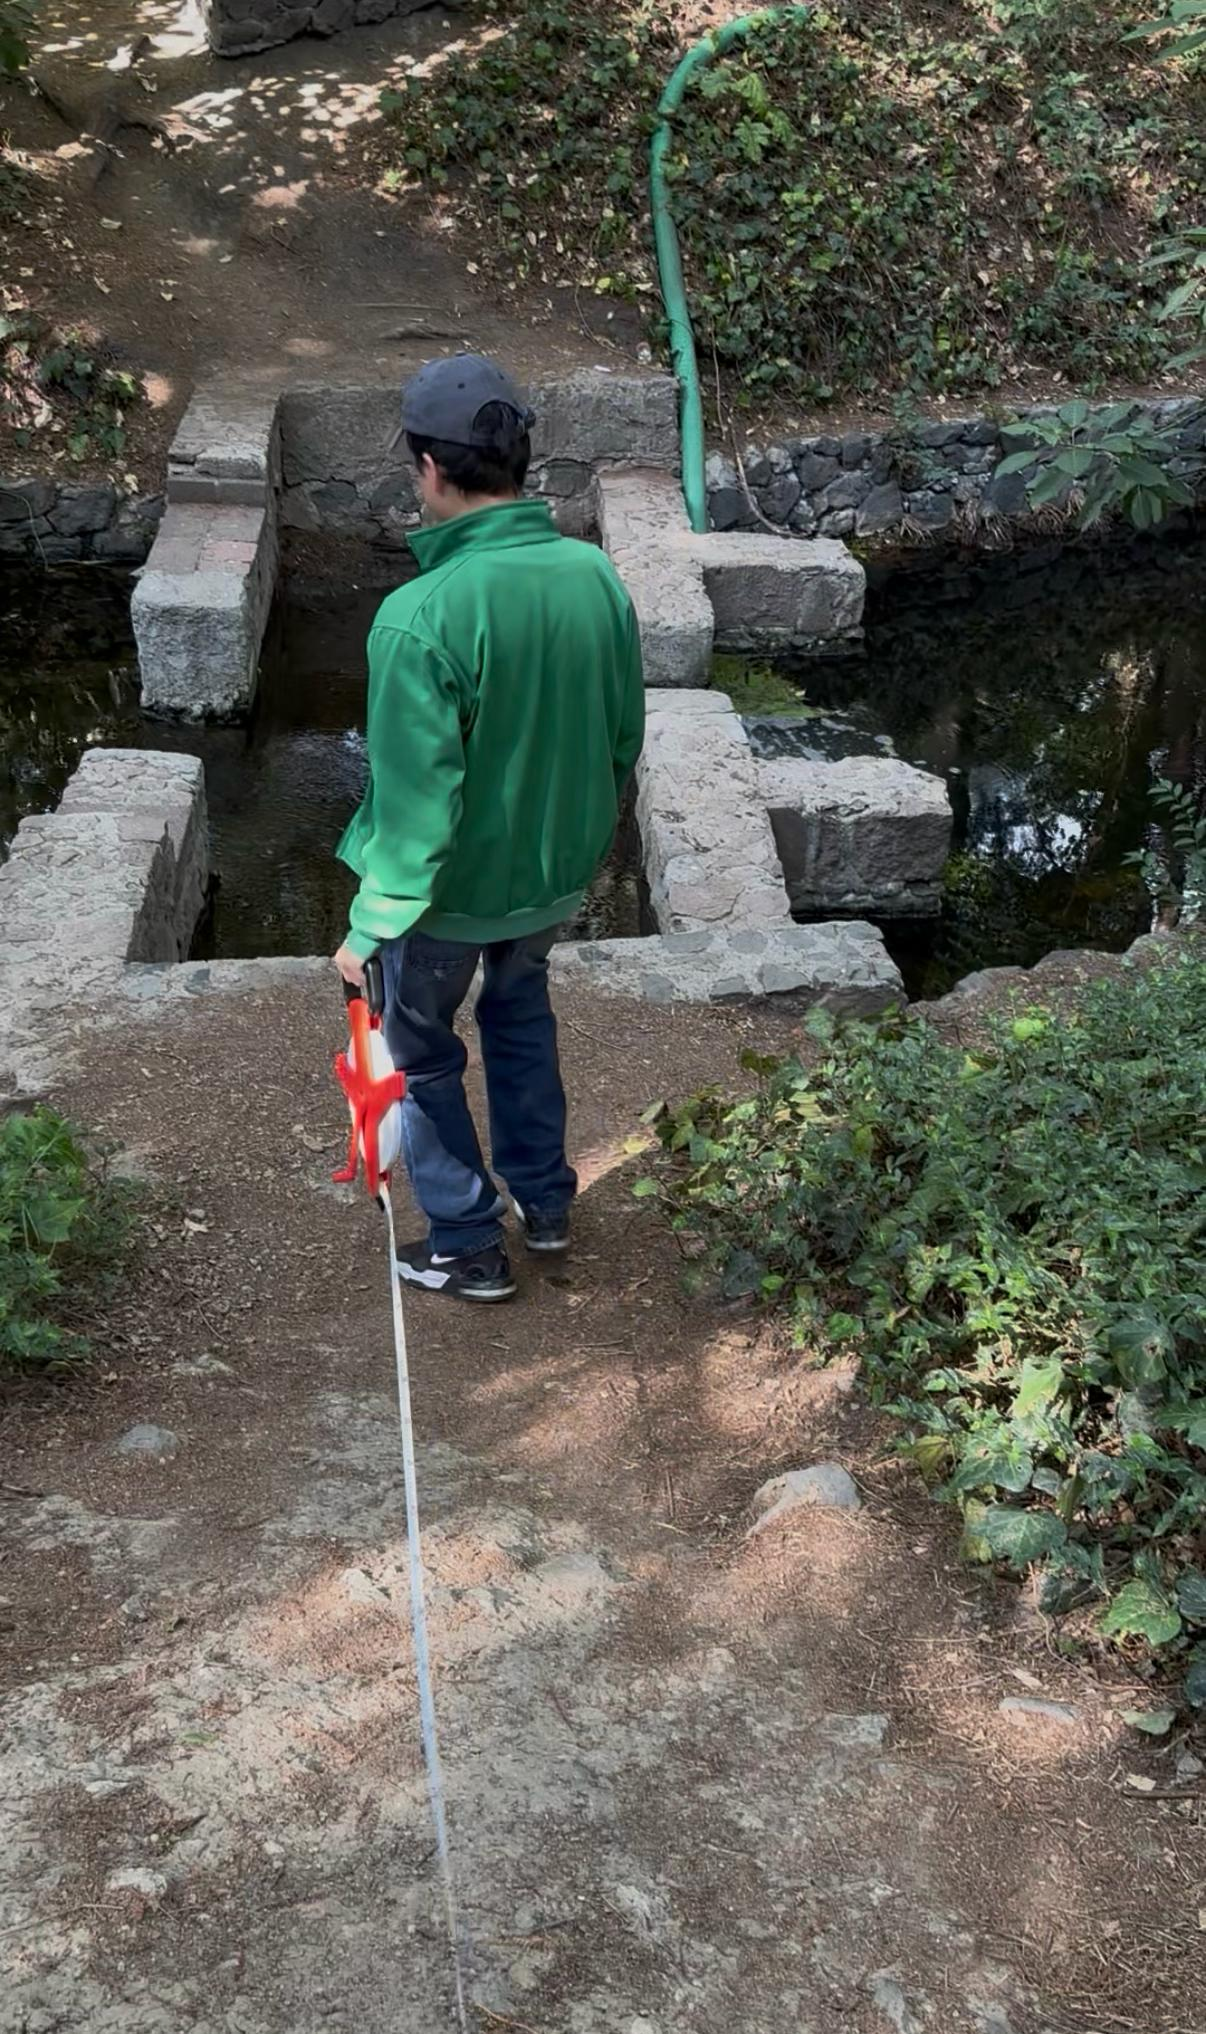
\includegraphics[width=0.40\textwidth, height=0.45\textheight, keepaspectratio]{../../Archivos/Imagenes_Logos/E1.jpeg} &
        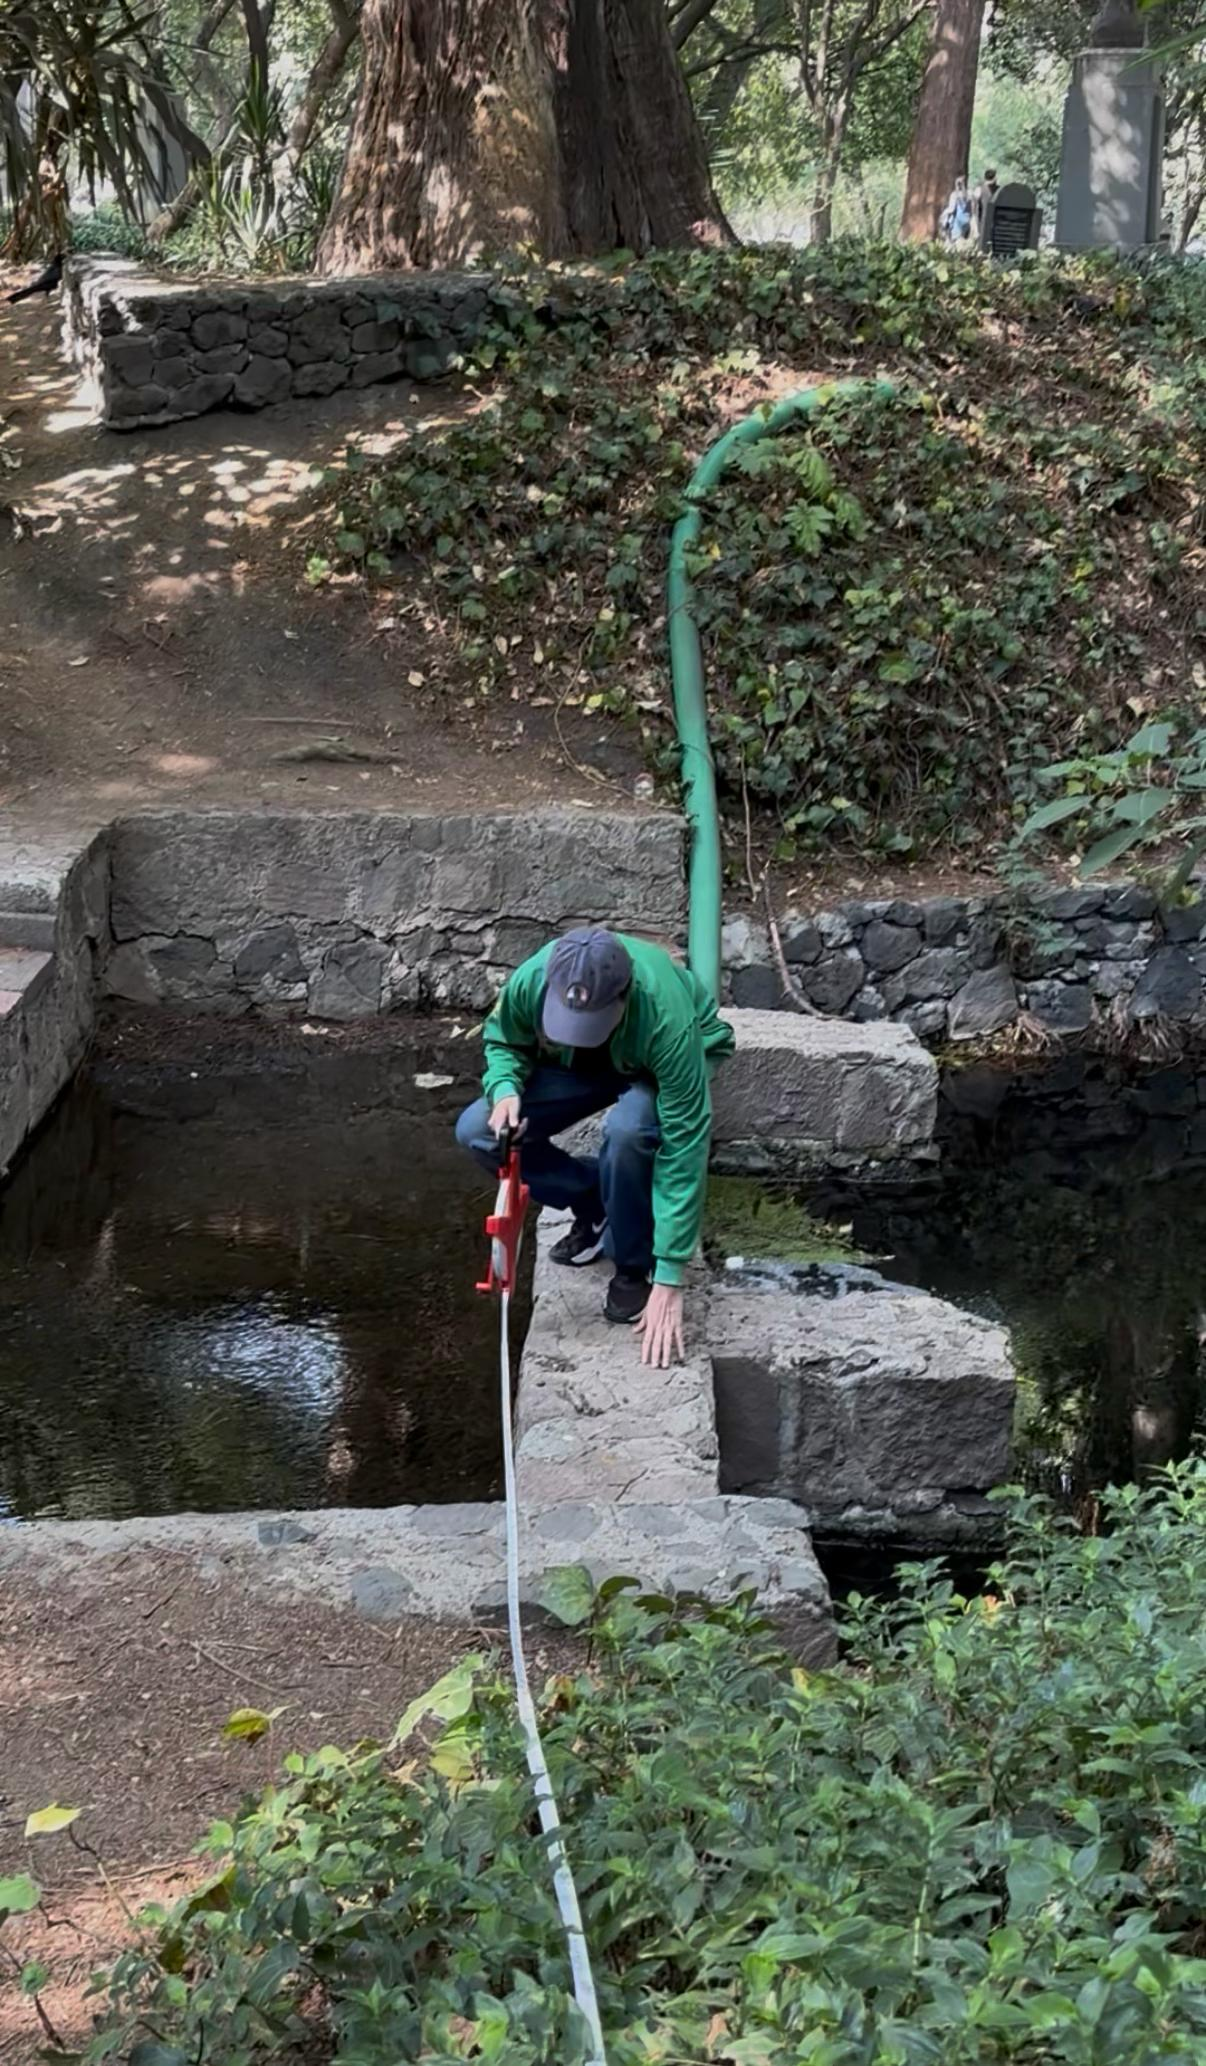
\includegraphics[width=0.40\textwidth, height=0.45\textheight, keepaspectratio]{../../Archivos/Imagenes_Logos/E2.jpeg} \\[0.3cm]
        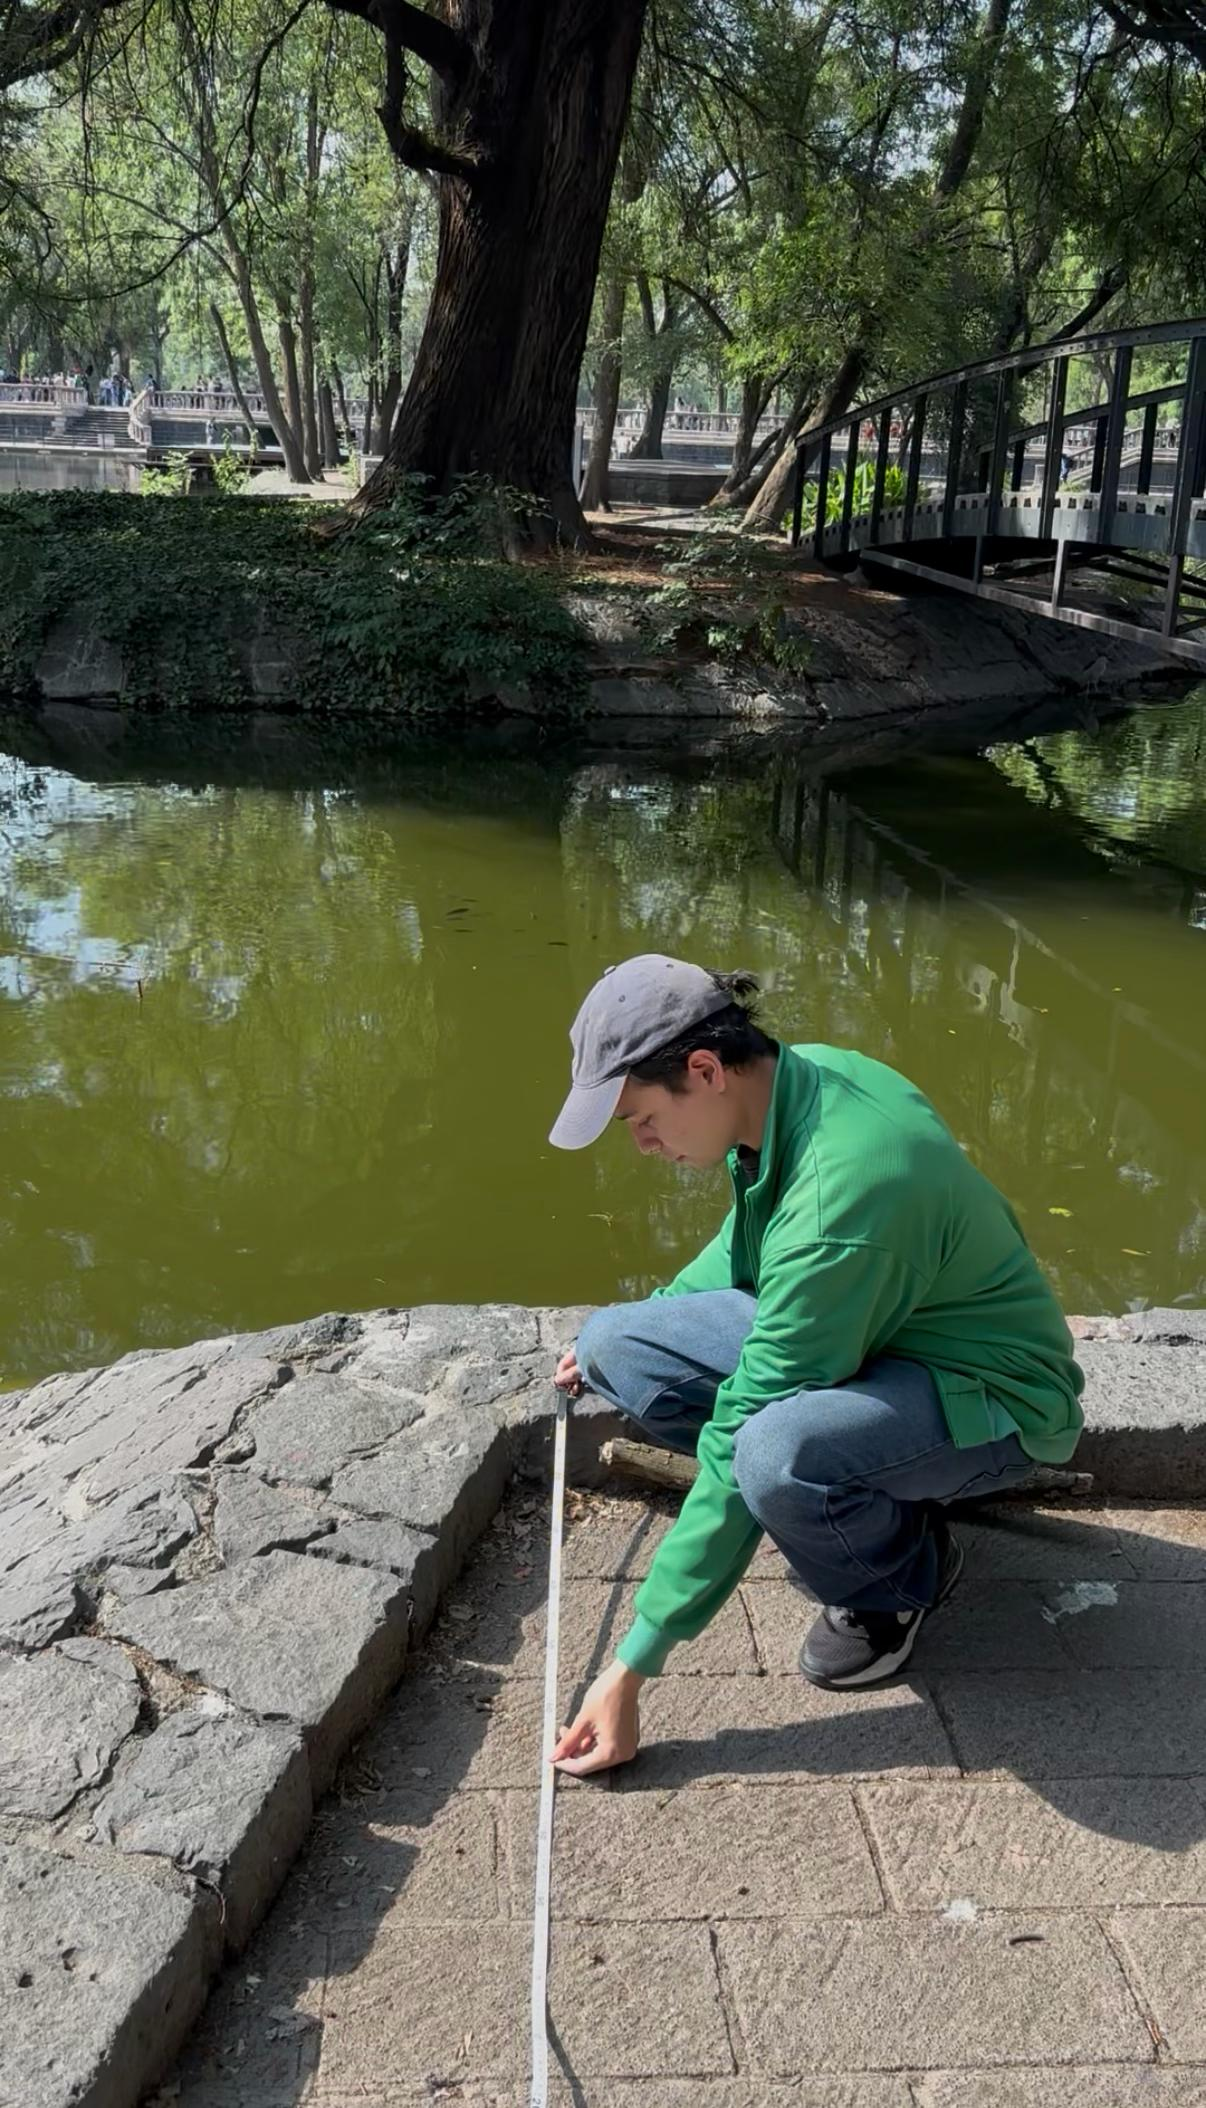
\includegraphics[width=0.40\textwidth, height=0.45\textheight, keepaspectratio]{../../Archivos/Imagenes_Logos/E3.jpeg} &
        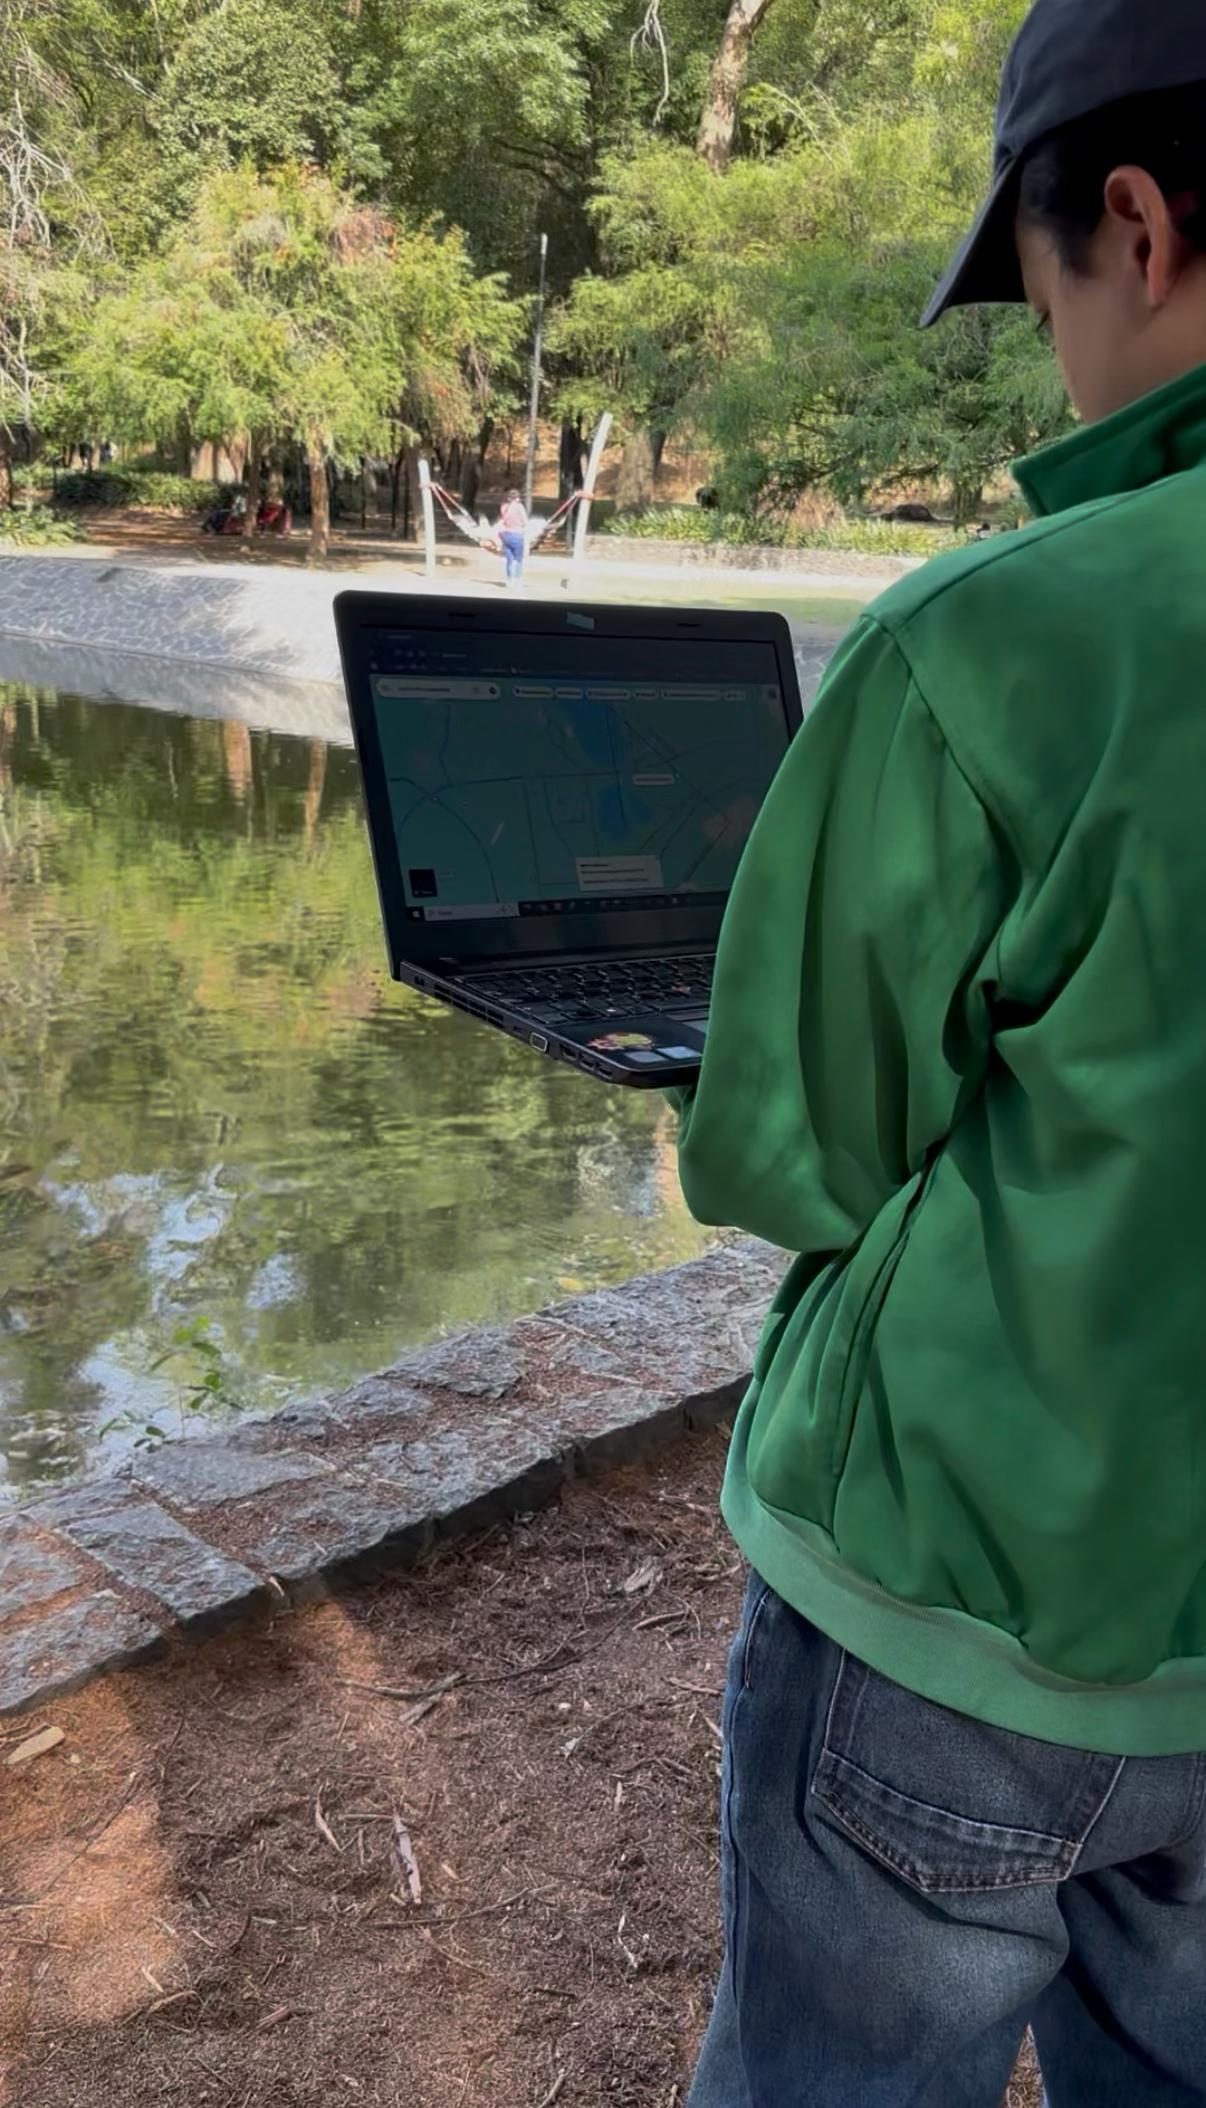
\includegraphics[width=0.40\textwidth, height=0.45\textheight, keepaspectratio]{../../Archivos/Imagenes_Logos/E4.jpeg}
\end{tabular}
    \end{center}
\end{frame}

\begin{frame}
    \frametitle{Evidencias de Trabajo de Campo}
    \begin{center}
        \begin{tabular}{cc}
        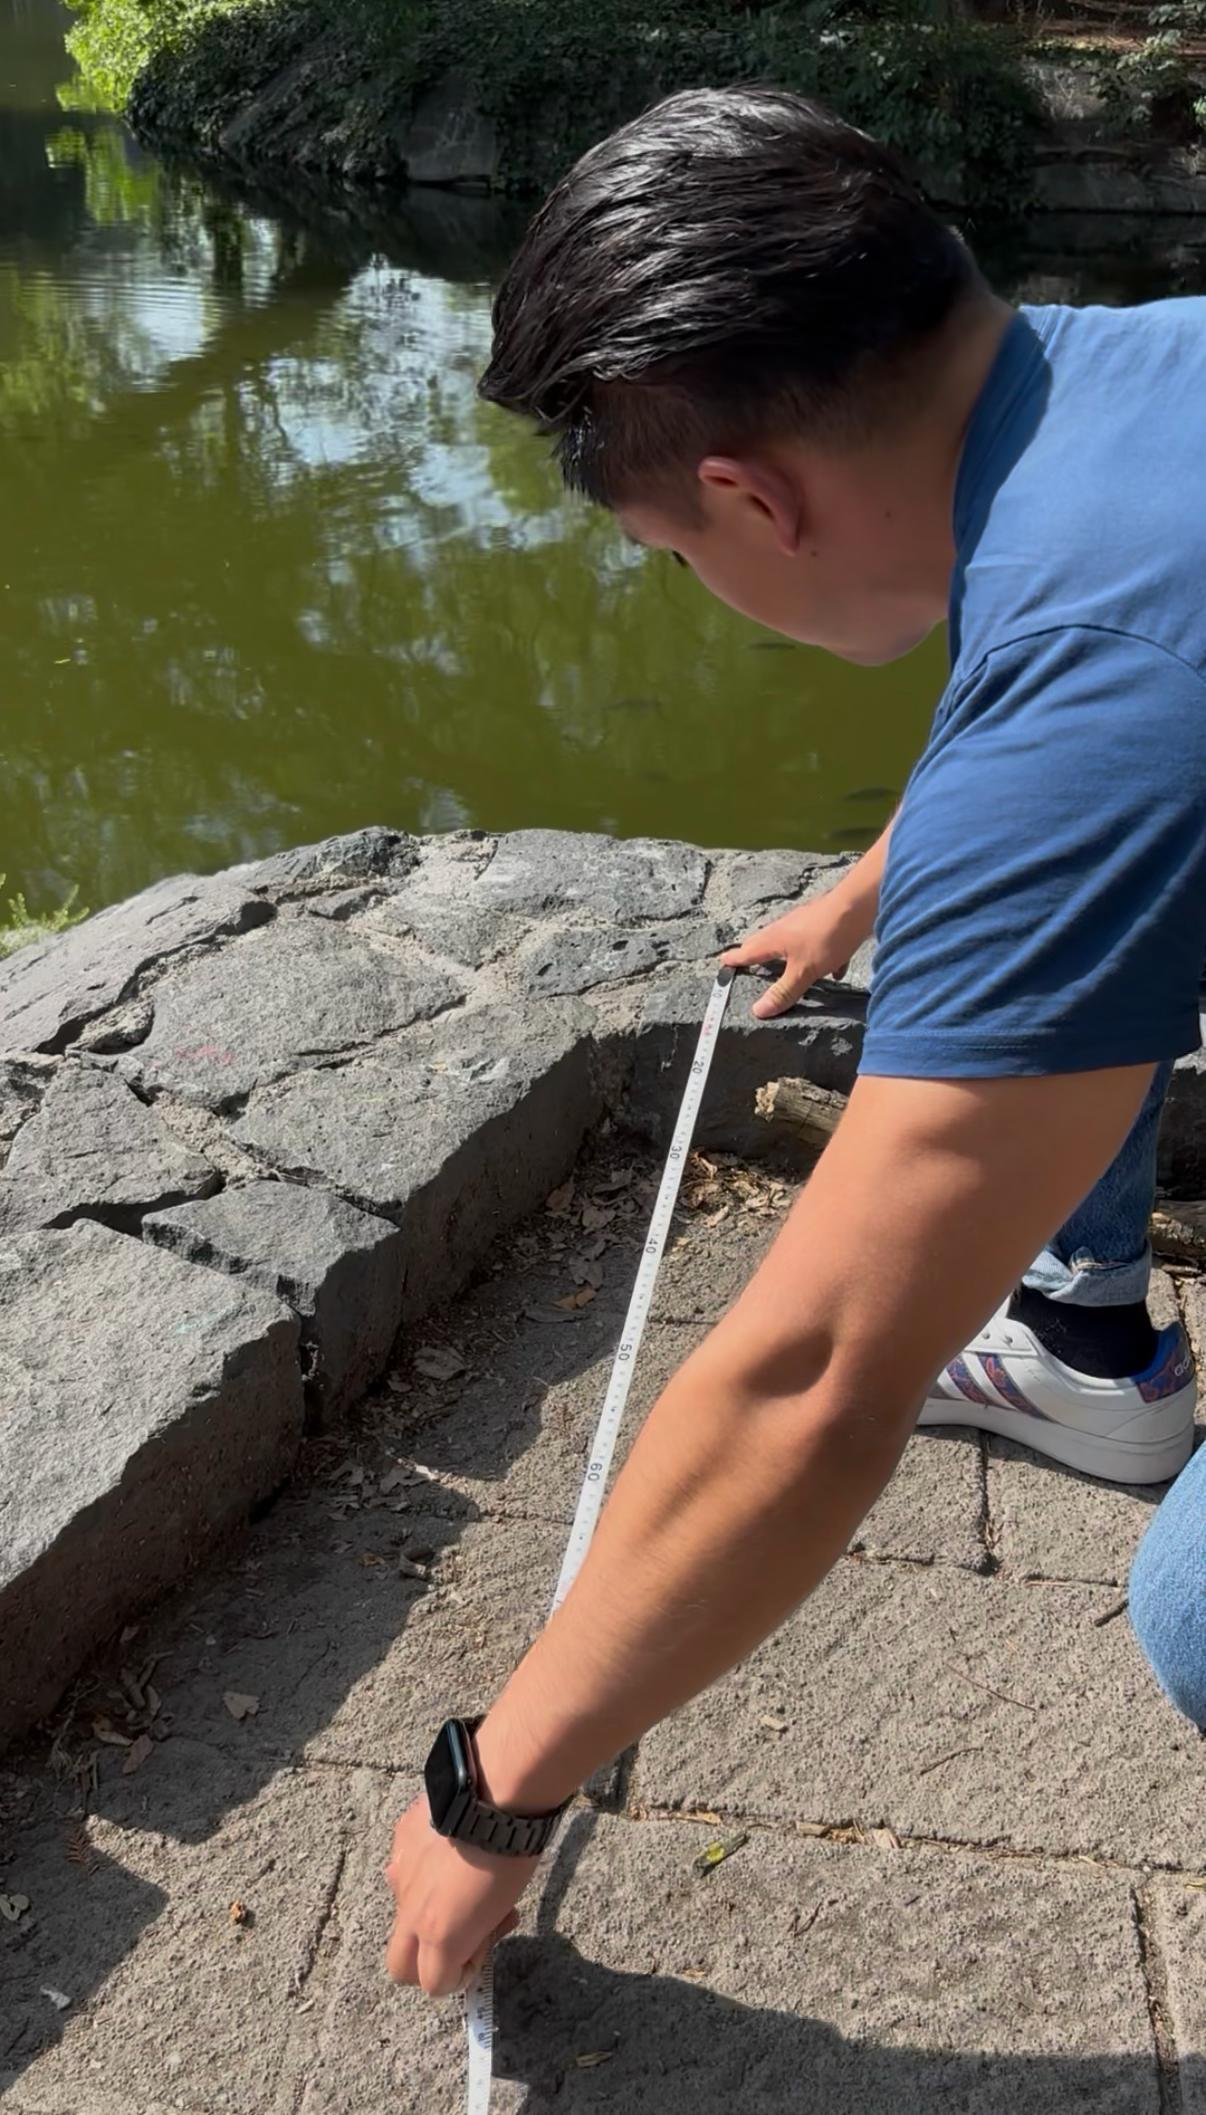
\includegraphics[width=0.40\textwidth, height=0.45\textheight, keepaspectratio]{../../Archivos/Imagenes_Logos/R1.jpeg} &
        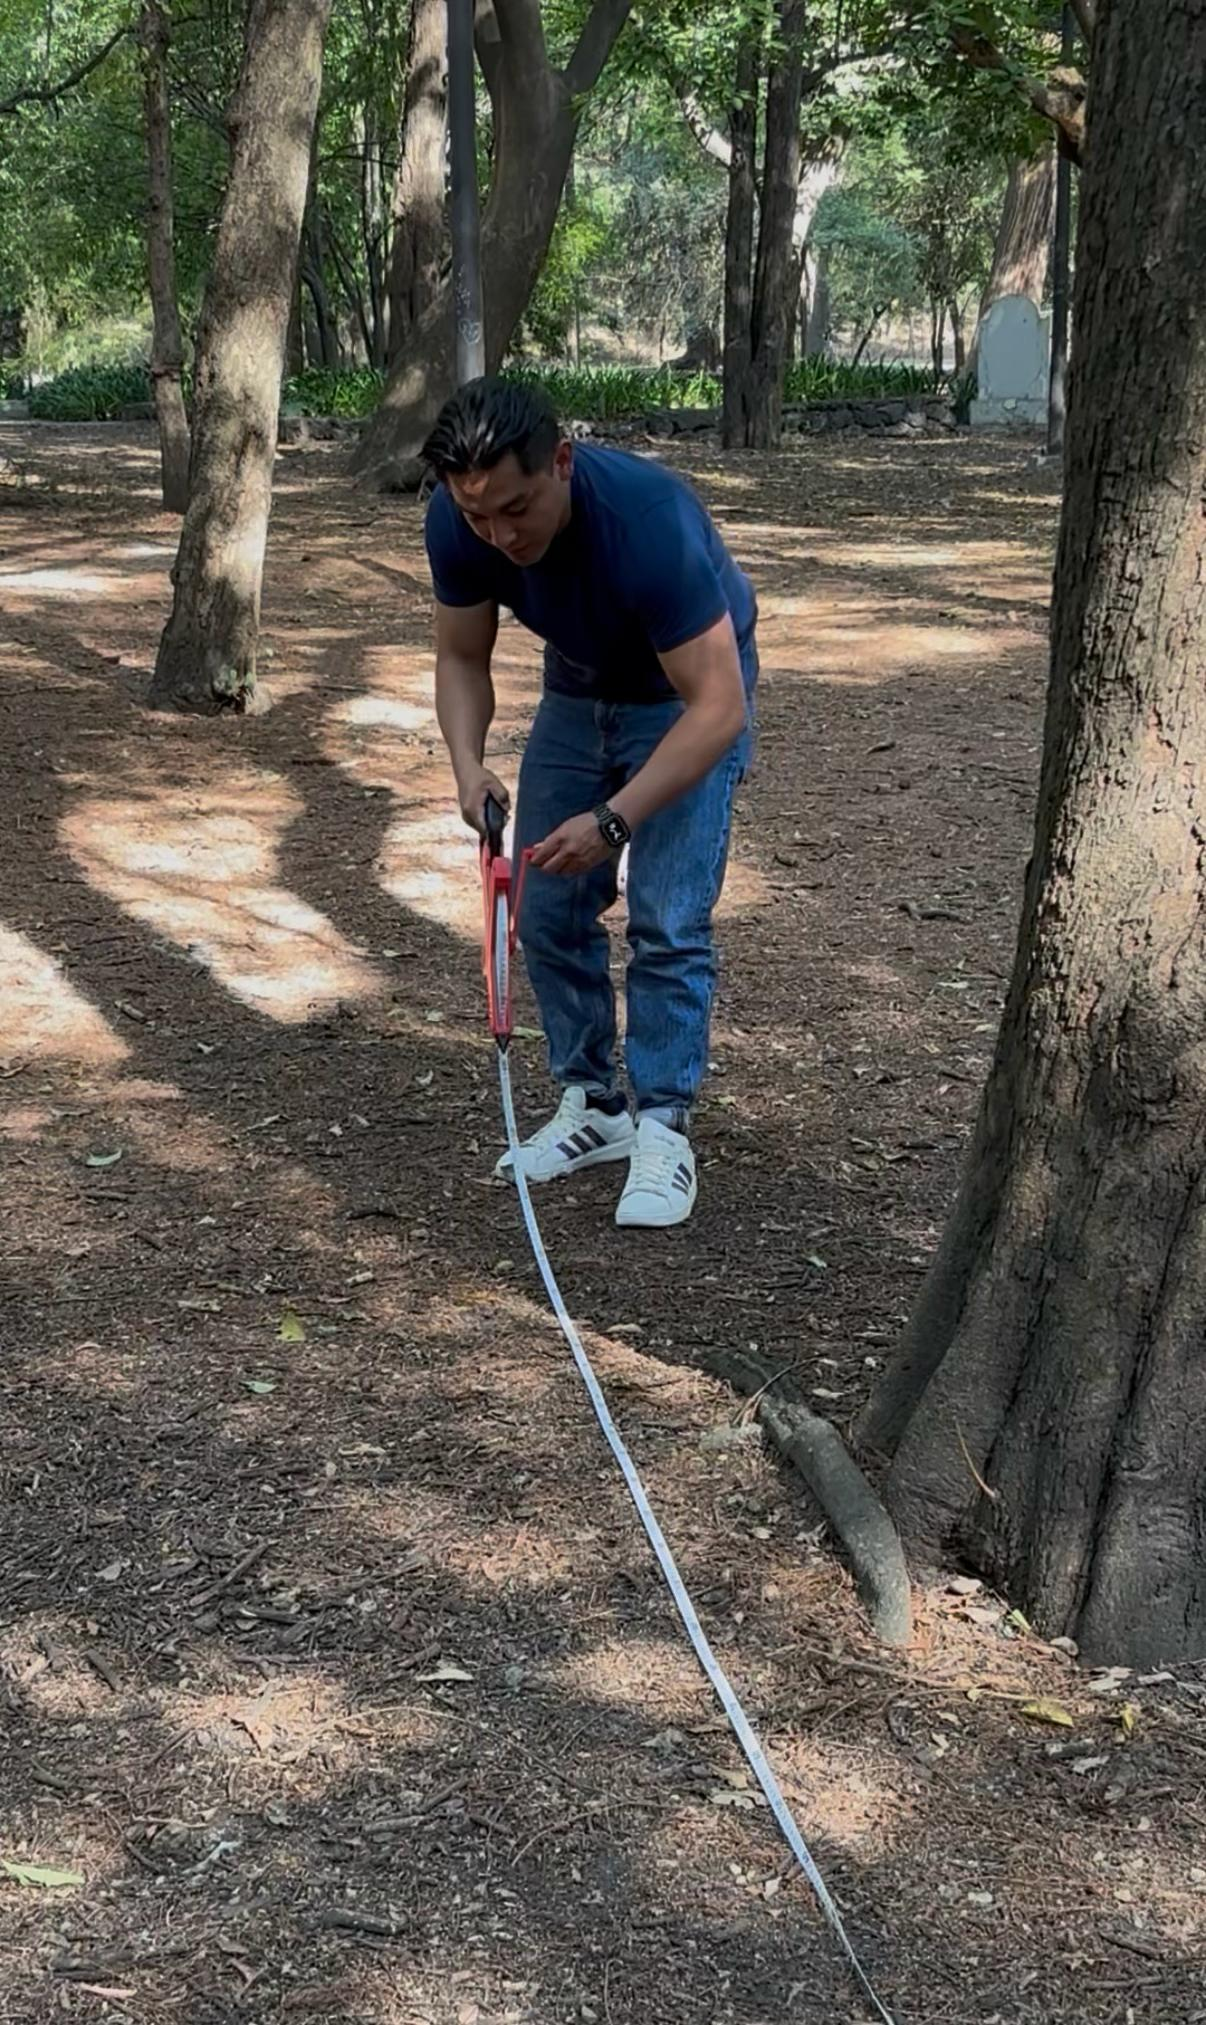
\includegraphics[width=0.40\textwidth, height=0.45\textheight, keepaspectratio]{../../Archivos/Imagenes_Logos/R2.jpeg} \\[0.3cm]
        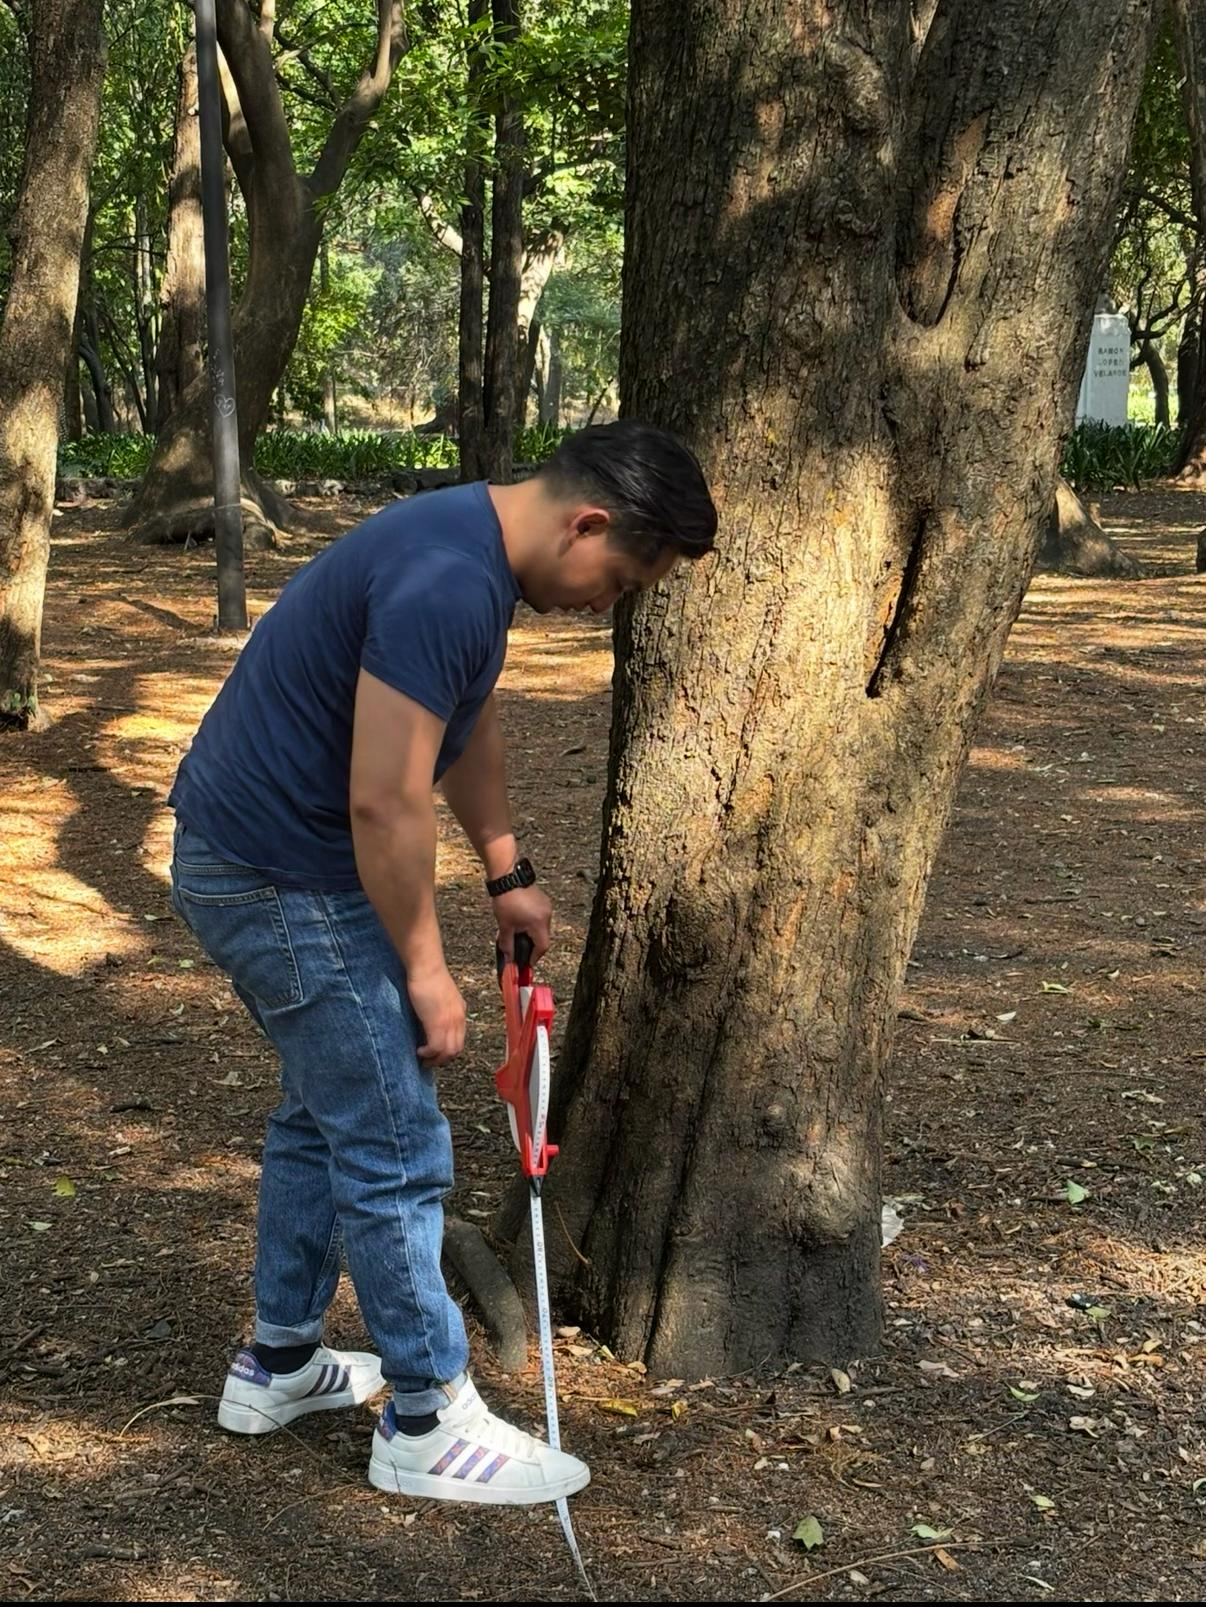
\includegraphics[width=0.40\textwidth, height=0.45\textheight, keepaspectratio]{../../Archivos/Imagenes_Logos/R3.jpeg} &
        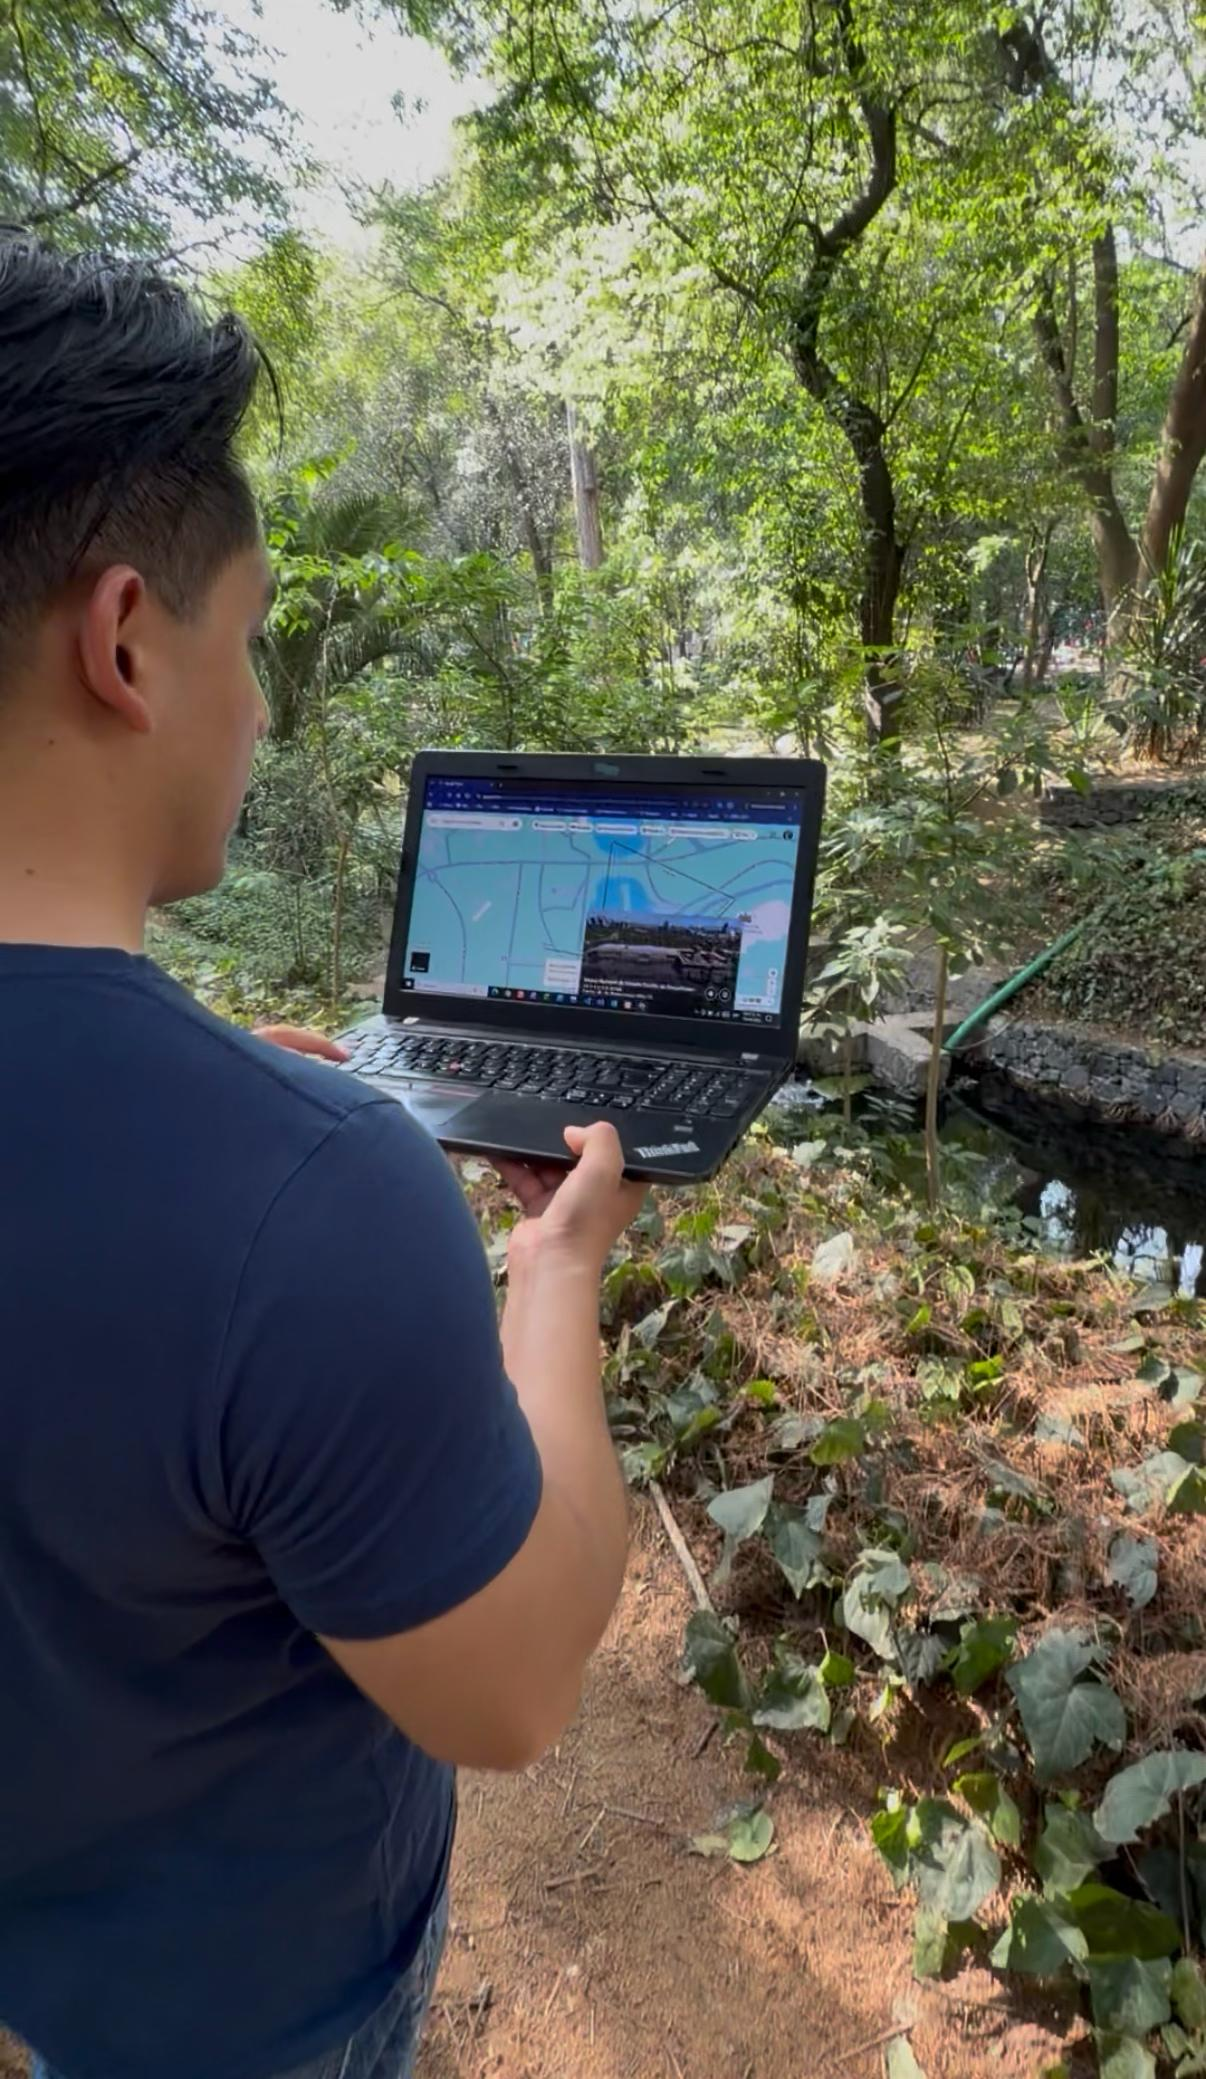
\includegraphics[width=0.40\textwidth, height=0.45\textheight, keepaspectratio]{../../Archivos/Imagenes_Logos/R4.jpeg}
\end{tabular}
    \end{center}
\end{frame}


\section{Referencias}


\begin{frame}[allowframebreaks]
    \frametitle{Referencias Bibliográficas (APA)}
    \begin{thebibliography}{99}
        
        \bibitem{taha2017} 
        Taha, H. A. (2017). 
        \newblock \textit{Investigación de operaciones} (10.ª ed.). 
        \newblock Pearson Educación.
        
        \bibitem{hillier2015} 
        Hillier, F. S., y Lieberman, G. J. (2015). 
        \newblock \textit{Introducción a la investigación de operaciones} (10.ª ed.). 
        \newblock McGraw-Hill.
        
        \bibitem{winston2004} 
        Winston, W. L. (2004). 
        \newblock \textit{Investigación de operaciones: Aplicaciones y algoritmos} (4.ª ed.). 
        \newblock Thomson.

        \bibitem{cormen2009}
        Cormen, T. H., Leiserson, C. E., Rivest, R. L., y Stein, C. (2009). 
        \newblock \textit{Introduction to algorithms} (3.ª ed.). 
        \newblock MIT Press.

    \end{thebibliography}
\end{frame}

\begin{frame}
    \frametitle{Fuentes Digitales}
    \textbf{Para la validación geoespacial y el procesamiento de datos:}
    \vspace{0.4cm}
    
    \begin{itemize}
        \item \textbf{Google Maps.} (2026). \textit{Ruta logística optimizada: Bosque de Chapultepec (N1 a N15)} [Mapa interactivo]. Recuperado de \url{https://www.google.com/maps}
        \vspace{0.3cm}
        \item \textbf{Google AI (Gemini).} (2026).[Modelo de lenguaje extenso].
        \vspace{0.3cm}
        \item \textbf{Proyecto Chapultepec Naturaleza y Cultura.} (2024). \textit{Infraestructura y movilidad en la Primera Sección} [Portal informativo]. Secretaría de Cultura.
    \end{itemize}
    
    \vspace{0.4cm}
    \textit{Nota: Las distancias y capacidades de la red fueron validadas mediante el software de análisis desarrollado.}
\end{frame}

\end{document}